\chapter{Tests}
\label{Tests}

Après l'écriture du code d'une application vient inévitablement cette étape que tous les développeurs craignent : les tests. Dans le cadre de mon projet tuteuré, elle s'est déroulé en trois phases biens distinctes.


\section{Validation par \og EDI Test Tool Kit \fg}
INTTRA met à disposition des développeurs un outil très utile : \og EDI Test Tool Kit \fg. Pour faire court, il s'agit d'un logiciel de validation de message (BL, Booking, etc.)

~

Son utilisation est simple et intuitive :
\begin{figure}[!ht]
	\begin{center}
		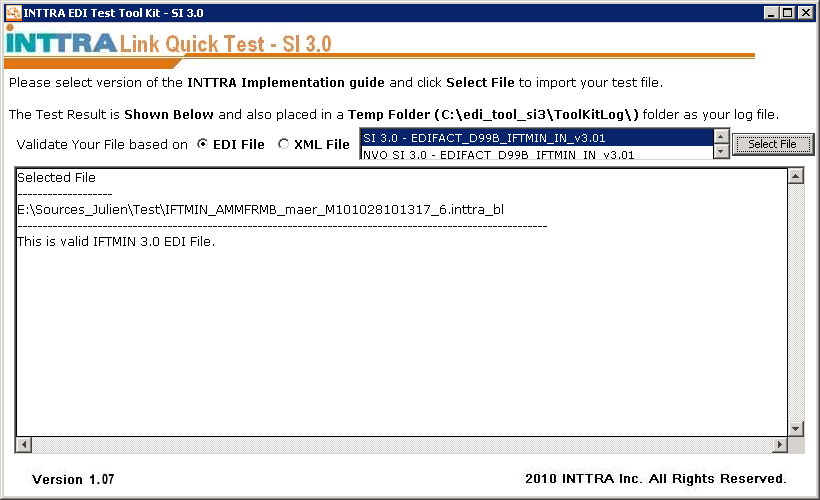
\includegraphics[scale=.85]{Contenu/ProjetTuteure/Images/EDI_Tools.png}
	\end{center}

	\caption{Utilisation de \og EDI Test Tool Kit \fg}
\end{figure}

Vous précisez le type de fichier, dans notre cas c'est donc \og EDI File \fg. Ensuite, dans la liste, vous sélectionnez la norme qui vous intéresse. Dans le cas des BL, il s'agit de \og D99B IFTMIN \fg.

Ensuite vous sélectionnez un fichier via le bouton et le programme vous avertit du résultat. En cas d'erreur, le numéro de la ligne est indiqué, ainsi qu'une description détaillée de l'erreur. Dans certains cas, le programme propose même des solutions.


\section{Avec un jeu d'essai}
Les premiers tests que j'ai menés ont été locaux. J'ai tenté de combler les failles les plus flagrantes de mon système en le testant avec des données sans queue ni tête.

~

Connaissant précisément le fonctionnement de l'application, j'ai été en mesure de prévoir des valeurs atypiques pour pousser le module dans ses derniers retranchements et valider son comportement. J'ai également comparé mon fichier et celui généré par \pireus{} afin de noter les différences et d'en déterminer l'origine.

~

Je n'ai pas rencontré de problèmes majeurs durant cette phase de test.


\section{Avec des données réelles}
La seconde phase a commencé seulement quelques jours après la fin de la première. Mon maître d'apprentissage, et je suis d'accord avec lui sur ce point, considère que les jeux d'essais construits à la main sont nécessaires, mais toujours insuffisants pour établir qu'un programme est pleinement fonctionnel.

Quelles que soient les précautions prises lors de la constitution des jeux d'essais, il suffit d'oublier un cas commun qui ne fonctionne pas pour paralyser les clients lors de la recette.

~

C'est pourquoi la second phase a consisté à me placer sur une session de \solulog{}, chez l'un de nos clients, pour tester l'application. Vu qu'il ne s'agissait pas encore de la phase de recette (qui est venue après), je n'ai pas opéré sur des documents en cours. J'ai utilisé la table d'audit pour ouvrir les informations correspondant à un cas déjà traité et comparer les résultats. J'ai procédé ainsi sur une période équivalente à un mois et demi de l'entreprise cliente.

~

L'énorme avantage de travailler ainsi est d'avoir accès à des données réelles et ainsi tester le programme sur les cas les plus communs. S'il se produit une erreur, elle est moins gênante si elle ne se produit que pour un BL sur plusieurs milliers, plutôt que si elle bloque plusieurs utilisateurs en même temps.

Même si je n'ai relevé aucune erreur flagrante, cette phase a néanmoins été très utile pour détecter quelques anomalies passées au travers des jeux de tests.

~

L'ensemble des tests a eu une durée approximative de deux jours complets.